\documentclass[11pt]{article}
\usepackage[margin=2.2cm]{geometry}
\usepackage{amsmath,amssymb,listings}
\usepackage{booktabs}
\usepackage{xurl}
\usepackage{xcolor}
\usepackage[colorlinks=true,linkcolor=blue!50!black,citecolor=blue!50!black,urlcolor=blue!50!black]{hyperref}
\usepackage{orcidlink}
\usepackage{tikz}
\usetikzlibrary{positioning,arrows.meta}
\usepackage{algorithm}
\usepackage{algpseudocode}

\lstset{
    language=Python,
    basicstyle=\ttfamily\small,
    keywordstyle=\color{blue!60!black}\bfseries,
    stringstyle=\color{green!45!black},
    commentstyle=\color{gray}\itshape,
    breaklines=true,
    frame=single,
    framerule=0.3pt,
    xleftmargin=1em,
    columns=fullflexible,
    keepspaces=true,
    showstringspaces=false
}
\lstdefinelanguage{lean4}{
    morekeywords={theorem,def,noncomputable,inductive,where,fun,namespace,end,
                  instance,set_option,Type,Prop},
    sensitive=true,
    morecomment=[l]{--},
    morestring=[b]"
}
\lstdefinestyle{lean}{
    language=lean4,
    basicstyle=\ttfamily\scriptsize,
    literate={∀}{{$\forall$}}1 {→}{{$\to$}}1 {⟨}{{$\langle$}}1 {⟩}{{$\rangle$}}1
             {λ}{{$\lambda$}}1
}
\lstdefinestyle{plain}{language={},basicstyle=\ttfamily\scriptsize}

\newcommand{\code}[1]{\texttt{#1}}
\newcommand{\lc}[1]{\texttt{#1}}
% py2tex emits \Return without a \State; give it a line of its own
\algrenewcommand\Return{\State \textbf{return} }

% every number below that describes a run is a macro written by that run
\input{gen/facts.tex}

\title{A Second Kernel Agrees:\\
``LEAN Proofs Small Enough to Read'',\\
Checked by Lean4 and Read Four Ways}
\author{Brent S. Hartshorn \orcidlink{0009-0004-2853-655X} \small \url{brenthartshorn@proton.me}}
\date{Supplementary material, September 2026}

\begin{document}
\maketitle

\begin{abstract}
Equation~(1) of \emph{LEAN Proofs Small Enough to Read} \cite{hartshorn2026lean}
states everything that paper proves about the \code{crustos} OS model as one
proposition, checked by the \code{lean4.py} micro-kernel. The micro-kernel
borrows Lean's design and its name, not its code. This supplement closes that
gap for the equation. A new exporter writes the kernel's terms as Lean~4
source, and Lean~\leanVersion{} checks them: the \leanDecls{} declarations the
equation depends on are accepted in \leanSeconds\,s, and
\code{\#print axioms} reports that the conjunction does not depend on any
axioms. Every other declaration in the environment is accepted too,
\leanAllDecls{} in all. The check is shown to be able to fail: changing one
word of the state invariant makes Lean refuse at exactly the proof step the
change breaks. Around that result, the equation is taken apart brace by brace
and given in four readings: the mathematics, the kernel's own \LaTeX{} (every
fragment reading back as the term it came from), Lean~4, and the Python it was
compiled from, both raw and as RosettaMath pseudocode. One script produces all
of it, and every number in this document is a macro written by the run that
measured it.
\end{abstract}

\section{Introduction}
\label{sec:intro}

The discussion of the main paper \cite{hartshorn2026lean} ended on the
observation that the Fermat formalization \cite{anthropic2026flt} was checked by a second,
independent kernel, ``precisely because the kernel is the only thing anyone
must believe''. The main paper's own kernel is \code{lean4.py}, a Calculus of
Constructions \cite{coquand1988} checker of 2{,}793 lines, part of RosettaMath \cite{hartshorn2026rosetta}, and the paper was careful to say
twice that it is not Lean \cite{demoura2021}. This supplement asks Lean anyway, in the form of release \leanVersion{} \cite{lean420}.

Its subject is one equation, reproduced here exactly as it appears in the main
paper's appendix:

\newcommand{\ctx}{\code{Ctx}}
\newcommand{\cur}[1]{#1.\code{cur}}
\newcommand{\nth}[1]{#1.\code{n}}
\newcommand{\hld}{\code{Holds}}

\begin{equation}
\label{eq:crustos}
\footnotesize
\begin{aligned}
&\overbrace{
  \underbrace{\forall c \in \ctx}_{\text{every state, not a tested one}},\;
  \hld\,\bigl(\underbrace{I}_{\lambda c,\ \code{leb}\,(\cur{c})\,(\nth{c})}\; c\bigr)
  \;\to\;
  \hld\,\bigl(I\;(\underbrace{\code{tick}\,(\code{sched}\,(\code{tick}\;c))}_{\code{run}\ =\ \text{three syscalls, proofs chained}})\bigr)
}^{\textbf{the state layer}}
\\[2.2ex]
&\hspace{3em}\text{where}\quad
\code{sched}\;c \;=\;
\underbrace{
  \code{Nat.rec}\;(\lambda n,\ \ctx \to \ctx)\;(\lambda s,\ s)\;\code{step}\;
  \underbrace{(\code{rank}\ c)}_{\code{sub}\,(\nth{c})\,(\cur{c})}\;c
}_{\code{sched.loop1}:\ \text{the variant bounds the passes, so the fold is the loop}}
\\[2.2ex]
&\hspace{3em}\phantom{\text{where}}\quad
\code{step} \;=\;
\lambda k\ \mathit{ih}\ s,\ \mathit{ih}\,\bigl(\code{ite}\;\ctx\;
    \underbrace{(\code{cond}\ s)}_{\code{ltb}\,(\cur{s})\,(\nth{s})}\;
    (\code{pass}\ s)\;s\bigr)
\\[2.2ex]
&\;\wedge\;
\overbrace{
  \forall\,\mathit{ns}\;\mathit{us},\;
  \hld\,\Bigl(\code{leb}\;
    \bigl(\code{len}\;\underbrace{(\code{accepted}\;\mathit{ns}\;\mathit{us})}_{\text{a \code{while} carrying a } \code{Prod}}\bigr)\;
    \bigl(\code{len}\;(\underbrace{\code{split}\;\mathit{us}\;44}_{44\ \text{is}\ \code{,}})\bigr)\Bigr)
}^{\textbf{the routing layer}}
\end{aligned}
\end{equation}

The first conjunct says the scheduler's state invariant survives three
composed syscalls, for every state. The second says the router's result is
never longer than its input, for every input. Their conjunction is one term of
type \code{Prop}, and both kernels have now checked a proof of it.

\paragraph{Contributions.}
\begin{itemize}
\item \textbf{A second kernel agrees} (\S\ref{sec:lean}). \code{leanexport.py}
  writes kernel terms as Lean~4 source. Lean~\leanVersion{} accepts the
  equation's \leanDecls{} declarations in \leanSeconds\,s with no axioms, and
  the whole environment, \leanAllDecls{} declarations. A tampered copy is
  refused where the tampering bites.
\item \textbf{The equation, brace by brace} (\S\ref{sec:braces}): each
  overbrace and underbrace of~(\ref{eq:crustos}) expanded into what
  it abbreviates, with the matching Lean~4 given braces of its own.
\item \textbf{Four readings, one generator} (\S\ref{sec:four},
  \S\ref{sec:python}): the kernel's \LaTeX{}, Lean~4, Python, and
  pseudocode, all written by \code{crustos\_eq.py} from the same environment.
  \rtFragments{} fragments of the equation, and all \rtEnvTerms{} types and
  values in the environment, read back as the terms they came from.
\end{itemize}

\begin{figure}[h]
\centering
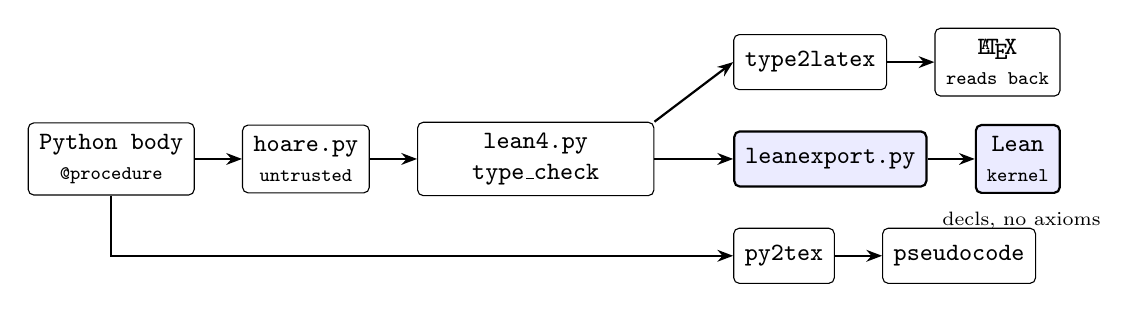
\begin{tikzpicture}[
  node distance=5mm and 6mm,
  box/.style={draw,rounded corners=2pt,inner sep=4pt,font=\small\ttfamily,minimum height=7mm,align=center},
  hot/.style={box,fill=blue!8,thick},
  lab/.style={font=\scriptsize,align=center},
  arr/.style={-{Stealth[length=2mm]},thick}]
  \node[box] (py) {Python body\\{\scriptsize @procedure}};
  \node[box,right=of py] (hoare) {hoare.py\\{\scriptsize untrusted}};
  \node[box,right=of hoare,minimum width=30mm] (env) {lean4.py\\type\_check};
  \node[box,above right=4mm and 10mm of env] (t2l) {type2latex};
  \node[hot,right=10mm of env] (lx) {leanexport.py};
  \node[box,below right=4mm and 10mm of env] (p2t) {py2tex};
  \node[box,right=of t2l] (tex) {\LaTeX{}\\{\scriptsize reads back}};
  \node[hot,right=of lx] (lean) {Lean \leanVersion\\{\scriptsize kernel}};
  \node[box,right=of p2t] (alg) {pseudocode};
  \draw[arr] (py)--(hoare); \draw[arr] (hoare)--(env);
  \draw[arr] (env.north east)--(t2l.west); \draw[arr] (env)--(lx);
  \draw[arr] (py.south) |- (p2t.west);
  \draw[arr] (t2l)--(tex); \draw[arr] (lx)--(lean); \draw[arr] (p2t)--(alg);
  \node[lab,below=1mm of lean] {\leanDecls{} decls, no axioms};
\end{tikzpicture}
\caption{One environment, three printers. The shaded path is new: the same
terms \code{type\_check} accepted, handed to a kernel nobody here wrote.}
\label{fig:pipeline}
\end{figure}

\section{The second kernel}
\label{sec:lean}

\subsection{Why ask}

A kernel is trusted because it is small enough to read, but reading is not
the only check available. Two kernels built independently, in different
languages, by different people, fail in different ways; a term both accept is
in much less doubt than a term either accepts. That is the reason the Fermat
formalization was run through a second checker, and it applies with more
force to \code{lean4.py}, which has one author.

It also tests a specific trusted-base extension. The main paper lists nine
literal accelerators as trusted Python: \code{normalize} takes their word on
numerals. The Lean export does not contain them. It writes each accelerated
name with the definition the accelerator stands in for, so Lean checks
\leanAccelerated{} as \code{Nat.rec} terms and nothing else. For the
equation, the second kernel does not rest on the accelerators at all.

\subsection{The translation}
\label{sec:translation}

A kernel term is already fully elaborated: every implicit argument is written
out, every binder carries its type, and there are no holes. So the export is a
printer, not a compiler, and Table~\ref{tab:translation} is the whole of it.

\begin{table}[h]
\centering
\tiny
\begin{tabular}{p{4.3cm}p{4.3cm}p{6.4cm}}
\toprule
\code{lean4.py} & Lean 4 & why \\
\midrule
$\Pi$, $\lambda$ over de Bruijn indices & \code{$\forall$ (x : A), B}, \code{fun (x : A) => b} & names chosen capture-free, as \code{type2latex} does; an unused $\lambda$ binder is \code{\_} \\
\code{Universe(0)}, \code{Universe(1)} & \code{Prop}, \code{Type} & no universe polymorphism to translate \\
\code{Nat}, \code{Bool}, \code{Eq}, \code{List}, \ldots & re-declared in \code{namespace RM} & constructors in the kernel's order: \code{Bool.rec} takes \code{true} first in both \\
\code{succ}, \code{mk}, \code{refl} & \code{Nat.succ}, \code{Prod.mk}, \code{Eq.refl} & kernel constructor names are global \\
\code{T.rec}, \code{T.ind} & \code{@T.rec} & Lean's one recursor eliminates into \code{Sort u}; the motive fixes \code{u} \\
an applied constant & \code{f a b}, or \code{@f a b} & \code{@} only where Lean generated an implicit binder: recursors, and constructors of parametrised types \\
\code{succ (succ zero)} & \code{2} & an \code{OfNat} instance reads a literal into the unary \code{RM.Nat} \\
an accelerated name & its definition & Lean has no accelerators to trust \\
definition, theorem & \code{noncomputable def}, \code{theorem} & by whether the type is a \code{Prop}; recursors have no compiled code \\
\bottomrule
\end{tabular}
\caption{\code{leanexport.py}, in full.}
\label{tab:translation}
\end{table}

Binder names follow Lean's lexical rules rather than the \LaTeX{} reader's.
The \LaTeX{} reader takes only single letters, so \code{type2latex} writes
\code{sched.loop1}'s induction hypothesis as $y$; Lean keeps the hint
\code{it}. One rule is new: a local may not be named after the first segment
of a dotted global in its body. A binder called \code{sched} would make
\code{sched.loop1} a field access on it.

\subsection{The equation in Lean 4}

Here is the theorem as Lean receives it, with the braces of~(\ref{eq:crustos})
put back:

\begin{equation}
\label{eq:lean}
\footnotesize
\begin{aligned}
&\underbrace{\lc{theorem crustos :}}_{\text{Lean re-checks the declaration}}\;\;\lc{And}
\\[0.5ex]
&\quad\overbrace{\lc{($\forall$ (c : Context),}\;
  \lc{Holds (}\underbrace{\lc{Context.invariant}}_{I}\lc{ c)}\;\to\;
  \lc{Holds (Context.invariant (}\underbrace{\lc{run c}}_{\lc{tick (sched (tick c))}}\lc{)))}}^{\textbf{the state layer}:\ \code{run\_preserves}}
\\[1ex]
&\quad\overbrace{\lc{($\forall$ (names : List (List Nat)) (urls : List Nat),}}^{\textbf{the routing layer}:\ \code{accepted\_bounded}}
\\[0.3ex]
&\qquad\lc{Holds (leb (len }\underbrace{\lc{Nat}}_{\text{implicit in (1)}}\lc{ (accepted names urls))}\;
  \lc{(len (List Nat) (}\underbrace{\lc{split urls 44}}_{44\ \text{is}\ \code{,}}\lc{))))}
\\[1ex]
&\underbrace{\lc{:= @And.conj}\;\ldots\;\lc{run\_preserves accepted\_bounded}}_{\text{the proof: two theorems, paired}}
\end{aligned}
\end{equation}

Three differences from~(\ref{eq:crustos}), none of them in the mathematics.
Lean writes \code{run} where the equation unfolds it; the two statements are
definitionally equal, and the driver checks that they are
(result: \unfoldedAgrees). The element type of \code{len} is an argument, because a
kernel term has no implicit arguments to hide. And the proof is visible: a
conjunction is built by \code{And.conj}, which takes the two propositions and
then one proof of each. \code{And} is the one declaration the main paper did
not need: its appendix called the conjunction ``a proposition the kernel
checks'', and the driver makes that literal by declaring it
(Listing~\ref{lst:and}).

\begin{lstlisting}[style=lean,caption={The conjunction, as exported. The whole proof is the last line.},label={lst:and}]
inductive And (P : Prop) (Q : Prop) : Prop where
  | conj : P → Q → And P Q

theorem crustos :
    And (∀ (c : Context), Holds (Context.invariant c) → Holds (Context.invariant (run c)))
        (∀ (names : List (List Nat)) (urls : List Nat),
           Holds (leb (len Nat (accepted names urls)) (len (List Nat) (split urls 44)))) :=
  @And.conj (...) (...) run_preserves accepted_bounded
\end{lstlisting}

\subsection{What Lean said}
\label{sec:verdict}

\begin{table}[h]
\centering
\small
\begin{tabular}{lr}
\toprule
declarations in the equation's closure & \leanDecls \\
lines of Lean 4 (\code{CrustOS.lean}) & \leanLines \\
characters & \leanChars \\
Lean version & \leanVersion \\
accepted & \leanOk \\
time to check, median of three runs & \leanSeconds\,s \\
\code{\#print axioms crustos} & \leanAxioms \\
\code{\#print axioms} on \code{crustos} and both termination theorems & \leanAxiomFree{} of 3 axiom-free \\
whole environment exported and accepted & \leanAllDecls{} declarations: \leanAllOk \\
not exported & \leanAllSkipped \\
\bottomrule
\end{tabular}
\caption{The second kernel's verdict. \code{Real} is an opaque constant with no
definition; nothing in the equation mentions it, and exporting it would mean
exporting an assumption.}
\label{tab:verdict}
\end{table}

The \code{\#print axioms} line is the one to read. Lean ships with three
axioms: propositional extensionality, the axiom of choice, and quotient
soundness. It also reports \code{sorryAx} whenever a proof was left
unfinished or failed to check. None appear. The conjunction, the two theorems
it pairs, both termination theorems (each reports the same), every lemma of
the main paper's Table~4 (\code{absurd} through \code{fold\_terminates}), and
every definition down to \code{Nat.rec} were checked from the definitions
alone. That is the claim the main paper made for \code{lean4.py}, now made by
a kernel it did not write.

The sizes of the proofs, as Lean sees them, are in Table~\ref{tab:proofsizes}.
\code{accepted\_bounded} is the largest: the case split on the \code{Prod}
the loop carries, then on the \code{ite} its \code{if} left behind, spelled
out in full.

\begin{table}[h]
\centering
\small
\begin{tabular}{lr}
\toprule
proof term & characters of Lean \\
\midrule
\code{crustos} & \proofCharsCrustos \\
\code{loop\_preserves} & \proofCharsLooppreserves \\
\code{tick\_preserves} & \proofCharsTickpreserves \\
\code{run\_preserves} & \proofCharsRunpreserves \\
\code{sched\_terminates} & \proofCharsSchedterminates \\
\code{fold\_terminates} & \proofCharsFoldterminates \\
\code{accepted\_bounded} & \proofCharsAcceptedbounded \\
\bottomrule
\end{tabular}
\caption{Proof terms as exported. Composition is cheap: \code{run\_preserves}
is little more than the three proofs it chains, inlined.}
\label{tab:proofsizes}
\end{table}

\subsection{A check that can fail}
\label{sec:tamper}

An acceptance means little unless the checker is shown refusing something.
The driver therefore makes one change to the exported file and runs Lean
again. It replaces \code{leb} with \code{ltb} in \code{Context.invariant},
which turns the invariant $\mathit{current} \le \mathit{nthreads}$ into
$\mathit{current} < \mathit{nthreads}$. The scheduler's exit state breaks the
new invariant, and so does its last pass. Lean refuses the copy, with
\tamperErrors{} errors, in \tamperWhere. The first error is:

\lstinputlisting[style=plain]{gen/lean-tampered.txt}

The error lands on the right step. In the case split on the one constructor
(\S7.1 of the main paper), \code{h2'2} is the hypothesis that the loop
condition held going in: $\mathit{current} < \mathit{nthreads}$, which is
\code{ltb}, which by definition is \code{leb (succ current) nthreads}. With
the original invariant, the invariant after one pass is that same
proposition, so the proof simply hands the hypothesis back. That was
\code{pass\_by\_cases} finding the goal ``by the condition''. With \code{ltb}
in the invariant, the goal after the pass becomes
$\mathit{current}+1 < \mathit{nthreads}$ and the hypothesis no longer fits.
Lean names exactly the term that stopped fitting. It then carries on past the
error, and says so: \code{\#print axioms} now reports ``\tamperAxioms''.

\subsection{What agreement does and does not show}
\label{sec:agreement}

The exporter is untrusted, like \code{hoare.py} and the elaborator. Suppose
it printed a different statement from the one \code{lean4.py} proved. Lean
would then have checked the wrong theorem, and nobody would be told. Two
things stand against that. The translation is a printer, one declaration per
declaration and one name per name (Table~\ref{tab:translation}), and its
output is readable: (\ref{eq:lean}) sits next to (\ref{eq:crustos}) above for
comparison. And every declaration down to \code{Nat} is exported, so the
statement's meaning is fixed by definitions Lean checked, not by names it was
given.

Agreement runs in one direction. Lean's definitional equality is larger than
\code{lean4.py}'s: it has proof irrelevance and $\eta$ for functions and
structures. So Lean accepting a term does not mean \code{lean4.py} would. The
direction tested here is the other one: everything \code{lean4.py} accepted,
Lean accepts too. Neither kernel knows what Python means. Both check the term
\code{hoare.py} produced, not the claim that the term is what the Python does,
and that step stays exactly as trusted as it was.

\section{The equation, brace by brace}
\label{sec:braces}

\subsection{The outer shape}

Remove the braces and (\ref{eq:crustos}) is $A \wedge B$, where $A$ and $B$
are each a $\Pi$-type. In the kernel it is one application, \code{And} to two
arguments, and \code{type2latex} writes it as:

\medskip
{\tiny\noindent$\input{gen/kt-crustos-type.tex}$}
\medskip

That is the kernel's own \LaTeX{}, typeset (\S\ref{sec:four} explains the one
change made for typesetting). The two overbraces of (\ref{eq:crustos}) are its
two arguments.

\subsection{\texorpdfstring{$\forall c \in \ctx$}{forall c in Ctx}: every state, not a tested one}

The main paper checked contracts two ways. \code{at(proc, value)} instantiates
the binder and settles the claim by computation: \code{refl} is the proof,
and it covers the value tested. A $\Pi$ is a claim about every \code{c}, and a
proof of it is a function that, handed any context and a proof that it
satisfies the invariant, returns a proof about \code{run c}. The underbrace
``every state, not a tested one'' marks the difference between those two
kinds of evidence. Only the second is what (\ref{eq:crustos}) states. In
Lean the binder reads \code{$\forall$ (c : Context)}, and \code{Context} is an
inductive type with one constructor and six fields
(Listing~\ref{lst:context}).

\subsection{\texorpdfstring{\code{Holds} and $I$}{Holds and I}: a contract is a Bool that computes to true}

\code{Holds} is the whole bridge from programs to propositions:
\[
  \code{Holds} \;:=\; \input{gen/kl-Holds-value.tex}
\]
The right-hand side is \code{type2latex} output, set as it was printed. The
printer writes \code{Eq Bool b true} as $b = \text{true}$ because the reader
would rebuild the same carrier from the binder's type. $I$ is
\code{Context.invariant}, and the underbrace in (\ref{eq:crustos}) is its
value with the projections shortened:
\[
  I \;=\; \input{gen/kt-Context-invariant-value.tex}
\]
In Lean:

\lstinputlisting[style=lean]{gen/lean-Context-invariant.lean}

\subsection{\texorpdfstring{\code{run}}{run}: three syscalls, proofs chained}

\code{run} is a definition, $\input{gen/kt-run-value.tex}$, and its
preservation proof is not a new argument. If \code{tick} hands the invariant
on and \code{sched} hands it on, their composition does, by applying the
proofs in turn:
\begin{equation}
\label{eq:chain}
\footnotesize
\lambda c\ h,\;
\underbrace{\mathit{tick}_{\mathrm{pf}}\;(\code{sched}\,(\code{tick}\,c))}_{\text{third step}}\;
\Bigl(
  \underbrace{\mathit{sched}_{\mathrm{pf}}\;(\code{tick}\,c)}_{\text{second step}}\;
  \bigl(\underbrace{\mathit{tick}_{\mathrm{pf}}\;c\;h}_{\text{first step: a proof about } \code{tick}\,c}\bigr)
\Bigr)
\end{equation}
Each proof takes a state and a proof about that state, and returns a proof
about the next state. Lean sees exactly this shape, with each
$\mathit{x}_{\mathrm{pf}}$ inlined as the case-split term
\code{preserves\_by\_cases} or \code{preserves\_by\_loop} built:

\lstinputlisting[style=lean,basicstyle=\ttfamily\tiny]{gen/lean-runpreserves-full.lean}

The outer \code{fun (c2 : Context) => @Context.rec \ldots} applied to
\code{(sched (tick c))} is $\mathit{tick}_{\mathrm{pf}}$ at the third step.
Its motive is the preservation statement, and its one case returns the
hypothesis unchanged, \code{=> h2}: \code{tick} changes only \code{ticks}, so
once the context is known to be a \code{Context.mk}, the invariant after is
literally the invariant before.

\subsection{The fold: five arguments to \texorpdfstring{\code{Nat.rec}}{Nat.rec}}
\label{sec:fold}

The \code{where} line is the heart of the equation, and the one place a
$\lambda$ cannot be avoided. \code{sched} is \code{sched.loop1}, and
\code{sched.loop1} applies \code{Nat.rec} to five arguments. The equation
braced only two; here are all five:
\begin{equation}
\label{eq:fold}
\footnotesize
\begin{aligned}
\code{sched.loop1}\;c \;=\;
\code{Nat.rec}\;
&\underbrace{(\lambda \_,\ \ctx \to \ctx)}_{\text{motive: }n\text{ passes give a state transformer}}\;\;
\underbrace{(\lambda s,\ s)}_{\text{zero passes: the identity}}
\\[1ex]
&\underbrace{(\lambda \_\ \mathit{it}\ s,\ \mathit{it}\,(\code{ite}\;\ctx\;(\code{cond}\,s)\;(\code{pass}\,s)\;s))}_{\text{one more pass: guard it, then run the rest}}\;\;
\underbrace{(\code{rank}\,c)}_{\text{fuel: the variant on entry}}\;\;
\underbrace{c}_{\text{the state}}
\end{aligned}
\end{equation}

Three points are easy to miss.

\emph{The motive returns a function.} \code{Nat.rec} does not build a
context; it builds a context transformer, $\ctx \to \ctx$, and the fifth
argument \code{c} is applied to what it returns. That is why the equation's
fold has a trailing \code{c}.

\emph{The step applies the rest last.} In \code{it (ite \ldots)}, the
induction hypothesis \code{it} (the transformer for $n$ passes) is applied
\emph{after} this pass, so $\code{iter}\,(n{+}1)\,s = \code{iter}\,n\,(\code{step}\,s)$.
The main paper explains why this is the right one of two definitions that
compute the same answer: the variant comes down on the first pass, so that is
where an induction on termination has to look.

\emph{Excess fuel is harmless.} \code{ite} runs \code{pass} only while
\code{cond} holds. Once it fails, each further pass returns \code{s}
unchanged; that fact is the lemma \code{stuck}. So running \code{rank c}
passes is enough when the variant bounds the number of real passes, and that
is \code{fold\_terminates}, whose Lean statement is:

\lstinputlisting[style=lean,basicstyle=\ttfamily\tiny]{gen/lean-foldterminates-statement.lean}

In Lean the fold reads almost the same as (\ref{eq:fold}). The recursor
is \code{@Nat.rec}, because its motive is implicit in Lean and explicit here:

\lstinputlisting[style=lean]{gen/lean-sched-loop1.lean}

\subsection{\texorpdfstring{\code{cond}, \code{pass}, \code{rank}}{cond, pass, rank}: the loop, in parts}

The loop's parts are separate definitions because a general lemma about folds
can only apply to a particular loop if that loop's parts have names. In the
kernel's own \LaTeX{}:
\begin{align*}
\code{sched.cond1} &= \input{gen/kt-sched-cond1-value.tex}\\
\code{sched.rank1} &= \input{gen/kt-sched-rank1-value.tex}
\end{align*}
\code{cond} is \code{ltb}, strictly less; the invariant is \code{leb}. That one
character is the whole story of \S\ref{sec:tamper}. \code{pass} is longer,
because two assignments to one context nest:

\lstinputlisting[style=lean]{gen/lean-sched-pass1.lean}

\code{c.current = c.current + 1} is a substitution in the compiler, so the
second statement, \code{c.ticks = c.ticks + 1}, reads \code{ticks} off the
already-updated context. Lean's version shows it: the inner
\code{Context.with\_current acc1 (\ldots)} appears twice.

\subsection{The routing layer: a \texorpdfstring{\code{while}}{while} carrying a \texorpdfstring{\code{Prod}}{Prod}}

The second conjunct looks simpler because its loop is hidden inside
\code{accepted}. \code{accepted}'s loop carries two variables, \code{out} and
\code{i}, so its state is a pair, and \code{accepted} is the first projection
of the loop's result:

\medskip
{\tiny\noindent$\code{accepted} \;=\; \input{gen/kt-accepted-value.tex}$}
\medskip

\noindent
The invariant is a conjunction over that pair. It is conjoined because
\code{i <= len(parts)} alone gives termination but not the result:

\lstinputlisting[style=lean,basicstyle=\ttfamily\tiny]{gen/lean-accepted-inv1.lean}

\code{urls} is a parameter of every part (\code{cond}, \code{pass},
\code{inv}, \code{rank}) because the loop's bound, \code{len (split urls 44)},
mentions it. The loop is a fold over the pair type, with exactly the five
arguments of (\ref{eq:fold}):

\lstinputlisting[style=lean,basicstyle=\ttfamily\tiny]{gen/lean-accepted-loop1.lean}

The underbrace ``44 is \code{,}'' is literal. \code{split} takes a byte and
44 is the byte for a comma, which in Lean arrives through the \code{OfNat}
instance as a unary \code{RM.Nat}. Nothing in the proof of
\code{accepted\_bounded} evaluates it, so the same proof would go through
for any separator.

\section{Four readings of one term}
\label{sec:four}

\subsection{The kernel's \LaTeX{} is \LaTeX{}}

\code{type2latex}'s output is a string in the \LaTeX{} subset
\code{latex2type} reads. It is written to be read back, not to be typeset, but
it is \LaTeX{} and can be typeset. One change is needed. To the reader, a space
is application: \code{\textbackslash text\{leb\} x} is \code{leb} applied to
\code{x}. To \TeX{} in math mode, a space is nothing, so it would print
``\code{lebx}''. The driver therefore writes each fragment twice:
\code{gen/kl-*.tex} is the printer's string, untouched, and
\code{gen/kt-*.tex} is the same string with each space made a visible,
breakable one. Listing~\ref{lst:raw} and the display under it are the same
term:

\lstinputlisting[style=plain,caption={\code{gen/kl-sched-loop1-value.tex}: \code{type2latex(value\_of(env, 'sched.loop1'))}, as printed.},label={lst:raw}]{gen/kl-sched-loop1-value.tex}

{\tiny\noindent$\input{gen/kt-sched-loop1-value.tex}$}
\medskip

\noindent Every fragment used here, \rtFragments{} in all, and every one of the
\rtEnvTerms{} types and values in the \envDecls-declaration environment,
satisfies $\code{latex2type}(\code{type2latex}(t)) = t$; failures:
\rtEnvFailed. (\ref{eq:crustos}) is these strings with names shortened, per
the main paper's Table~6. Because the driver builds a fresh environment in
which \code{tick} is declared once, the main paper's note about \code{tick2}
does not arise here.

\subsection{Side by side}

Table~\ref{tab:corr} is the index: each name in (\ref{eq:crustos}), what the
environment calls it, and where it comes from in Python.

\begin{table}[h]
\centering
\scriptsize
\begin{tabular}{llll}
\toprule
in (\ref{eq:crustos}) & kernel and Lean name & kernel \LaTeX{} (\code{gen/kl-}) & Python origin \\
\midrule
$\ctx$ & \code{Context} & (a name, printed as is) & \code{record(env, 'Context', ...)} \\
$\hld$ & \code{Holds} & \code{Holds-value} & \code{prelude()} \\
$I$ & \code{Context.invariant} & \code{Context-invariant-value} & \code{state\_invariant(env, 'Context', ...)} \\
$\cur{c}$, $\nth{c}$ & \code{Context.current}, \code{.nthreads} & \code{Context-current-value} & \code{c.current}, \code{c.nthreads} \\
\code{tick} & \code{tick} & \code{tick-value} & \code{def tick} \\
\code{run} & \code{run} & \code{run-value} & \code{compose(env, 'run', ...)} \\
\code{sched} & \code{sched}, \code{sched.loop1} & \code{sched-loop1-value} & the \code{while} in \code{def sched} \\
\code{cond} & \code{sched.cond1} & \code{sched-cond1-value} & \code{while c.current < c.nthreads} \\
\code{pass} & \code{sched.pass1} & \code{sched-pass1-value} & the loop body \\
\code{rank} & \code{sched.rank1} & \code{sched-rank1-value} & \code{assert variant(...)} \\
\code{accepted} & \code{accepted}, \code{accepted.loop1} & \code{accepted-value} & \code{def accepted} \\
\code{split} & \code{split} & \code{split-value} & \code{prelude()} \\
the conjunction & \code{crustos} & \code{crustos-type} & \code{L.define(env, 'crustos', ...)} \\
\bottomrule
\end{tabular}
\caption{One index for four readings. Lean uses the kernel's names unchanged,
except that constructors are qualified by their type.}
\label{tab:corr}
\end{table}

\section{The Python it came from}
\label{sec:python}

\subsection{Raw, and as pseudocode}

Everything above was compiled from four Python functions. Two are shown here
as written, each beside what \code{rosettamath.py2tex} makes of it. The
contract lives in the decorator, which \code{py2tex} does not represent and
says so with a comment rather than dropping it silently.

\noindent
\begin{minipage}[t]{0.45\textwidth}
\lstinputlisting[basicstyle=\ttfamily\tiny]{gen/py-sched.py}
\end{minipage}\hfill
\begin{minipage}[t]{0.53\textwidth}
\footnotesize
\input{gen/py2tex-sched.tex}
\end{minipage}

\medskip
\noindent
\begin{minipage}[t]{0.45\textwidth}
\lstinputlisting[basicstyle=\ttfamily\tiny]{gen/py-accepted.py}
\end{minipage}\hfill
\begin{minipage}[t]{0.53\textwidth}
\footnotesize
\input{gen/py2tex-accepted.tex}
\end{minipage}

\medskip
Reading the two columns against Table~2 of the main paper gives the lowering:
the \code{while} is the fold of (\ref{eq:fold}), the two \code{assert}s are
\code{inv} and \code{rank}, the loop body is \code{pass}, and the \code{if}
inside \code{accepted}'s loop is the \code{ite} its preservation proof splits
on.

\subsection{The return journey}

\code{py2tex} has an inverse, \code{tex2py}, and the driver runs both. The
restored function bodies are compared with the originals: \code{tick}
\pyRoundtripTick, \code{sched} \pyRoundtripSched, \code{scheme\_of}
\pyRoundtripSchemeof, \code{accepted} \pyRoundtripAccepted. The change in
\code{accepted} is instructive. The pseudocode writes
\code{out: 'Array' = []} as $\mathit{out} \gets []$ and the parameters without
annotations, and nothing else is lost: the restored function computes the
same thing. But it is no longer a function \code{hoare.py} will read. Handed
the restored source, the imperative fragment refuses:

\lstinputlisting[style=plain]{gen/hoare-accepted.txt}

All four restored functions are refused for the same reason. Pseudocode keeps
the behaviour and drops the types, and the types are what a proof needs:
without \code{'Strs'} there is no $\Pi$ to state, and without \code{'Array'}
an empty list has no element type. This is the same line the main paper
draws between a runtime check and a proof. The pseudocode is faithful as a
program and silent as a specification.

\subsection{How the proofs are assembled}

The proofs are Python calls that build kernel terms, and the kernel checks
each one as it is declared. For the state layer, the calls are:

\lstinputlisting[basicstyle=\ttfamily\tiny]{gen/driver-state.py}

For the routing layer, the preservation step is written out by hand: split on
the pair, split on the \code{ite}, and rejoin the conjunction with
\code{andb\_both}. The postcondition then follows from the invariant at exit:

\lstinputlisting[basicstyle=\ttfamily\tiny]{gen/driver-accepted.py}

Finally the conjunction, which is the step that makes (\ref{eq:crustos}) one
declaration:

\lstinputlisting[basicstyle=\ttfamily\tiny]{gen/driver-equation.py}

\section{Reproducing this document}
\label{sec:repro}

\begin{lstlisting}[style=plain]
python3 crustos_eq.py      # rebuilds the model, writes gen/ and CrustOS.lean,
                           # and runs lean on it if lean is on PATH
lean CrustOS.lean          # the second kernel, on its own
pdflatex crustos_eq.tex    # twice, for references
\end{lstlisting}
\small
The driver exits non-zero unless every fragment reads back, the unfolded
statement agrees with the declared one, Lean accepts the export, and Lean
refuses the tampered copy. Only Lean~\leanVersion{} has been tested. The
export uses no library, only \code{inductive}, \code{def}, \code{theorem}
and one \code{instance}, so other Lean~4 releases are expected to accept it,
but that has not been checked. The model builds in
\buildSeconds\,s. \code{CrustOS.lean} is written next to the driver and can be
committed with it, so that the second check needs no Python at all.

\section{Limits}
\label{sec:limits}
\small
\begin{itemize}
\item \textbf{The exporter is untrusted.} A mistranslation that still
  type-checked would make Lean check a different theorem.
  \S\ref{sec:agreement} gives the mitigations; they are mitigations, not a
  proof.
\item \textbf{Lean checks the terms, not the lowering.} That
  \code{sched.loop1} is what the Python \code{while} does is
  \code{hoare.py}'s claim, in both kernels.
\item \textbf{The literal instance is new code.} \code{ofNat} and its
  \code{OfNat} instance exist only on the Lean side. They are ordinary
  definitions that Lean checks, and nothing in the equation's proofs reduces
  a literal.
\item \textbf{Lean's equality is larger.} Acceptance by Lean does not predict
  acceptance by \code{lean4.py}; only the tested direction is claimed.
\item \textbf{Still a model.} As in the main paper, \code{crustos} is modelled,
  not booted.
\end{itemize}

\appendix
\section{The model's declarations in Lean 4}
\label{sec:appendix}

The data types, and the definitions (\ref{eq:crustos}) names, as exported.
Proofs are omitted here but are in \code{CrustOS.lean}.

\lstinputlisting[style=lean,basicstyle=\ttfamily\tiny]{gen/lean-Bool.lean}
\lstinputlisting[style=lean,basicstyle=\ttfamily\tiny]{gen/lean-Nat.lean}
\lstinputlisting[style=lean,basicstyle=\ttfamily\tiny]{gen/lean-Eq.lean}
\lstinputlisting[style=lean,basicstyle=\ttfamily\tiny]{gen/lean-Prod.lean}
\lstinputlisting[style=lean,basicstyle=\ttfamily\tiny]{gen/lean-List.lean}
\lstinputlisting[style=lean,basicstyle=\ttfamily\tiny,caption={The six-field record.},label={lst:context}]{gen/lean-Context.lean}
\lstinputlisting[style=lean,basicstyle=\ttfamily\tiny]{gen/lean-Context-current.lean}
\lstinputlisting[style=lean,basicstyle=\ttfamily\tiny]{gen/lean-Context-withticks.lean}
\lstinputlisting[style=lean,basicstyle=\ttfamily\tiny]{gen/lean-Holds.lean}
\lstinputlisting[style=lean,basicstyle=\ttfamily\tiny]{gen/lean-ite.lean}
\lstinputlisting[style=lean,basicstyle=\ttfamily\tiny]{gen/lean-leb.lean}
\lstinputlisting[style=lean,basicstyle=\ttfamily\tiny]{gen/lean-len.lean}
\lstinputlisting[style=lean,basicstyle=\ttfamily\tiny]{gen/lean-tick.lean}
\lstinputlisting[style=lean,basicstyle=\ttfamily\tiny]{gen/lean-sched-cond1.lean}
\lstinputlisting[style=lean,basicstyle=\ttfamily\tiny]{gen/lean-sched-rank1.lean}
\lstinputlisting[style=lean,basicstyle=\ttfamily\tiny]{gen/lean-sched.lean}
\lstinputlisting[style=lean,basicstyle=\ttfamily\tiny]{gen/lean-run.lean}
\lstinputlisting[style=lean,basicstyle=\ttfamily\tiny]{gen/lean-accepted-cond1.lean}
\lstinputlisting[style=lean,basicstyle=\ttfamily\tiny]{gen/lean-accepted-pass1.lean}
\lstinputlisting[style=lean,basicstyle=\ttfamily\tiny]{gen/lean-accepted-rank1.lean}
\lstinputlisting[style=lean,basicstyle=\ttfamily\tiny]{gen/lean-accepted.lean}
\lstinputlisting[style=lean,basicstyle=\ttfamily\tiny]{gen/lean-runpreserves-statement.lean}
\lstinputlisting[style=lean,basicstyle=\ttfamily\tiny]{gen/lean-acceptedbounded-statement.lean}
\lstinputlisting[style=lean,basicstyle=\ttfamily\tiny]{gen/lean-schedterminates-statement.lean}

\section*{Reproducibility --- Source Code}

\url{https://github.com/brentharts/RosettaMath} --- \code{crustos\_eq.py},
\code{leanexport.py}, \code{CrustOS.lean}

\footnotesize

\begin{thebibliography}{9}

\bibitem{hartshorn2026lean} Hartshorn, B.~S. (2026). LEAN Proofs Small Enough
to Read: Kernel Contracts from \LaTeX{} Theorems to Compiler Decisions.
\emph{ai.viXra} 2609.0019.
\url{https://ai.vixra.org/abs/2609.0019}

\bibitem{hartshorn2026rosetta} Hartshorn, B.~S. (2026). RosettaMath: Reading,
Running and Proving Mathematics from \LaTeX{}. SSRN.
\newline
\url{https://dx.doi.org/10.2139/ssrn.7435598}

\bibitem{demoura2021} de Moura, L., \& Ullrich, S. (2021). The Lean 4
theorem prover and programming language. In \emph{CADE 28}, LNCS 12699,
625--635.

\bibitem{lean420} Lean FRO (2025). Lean 4 v4.20.0.
\url{https://github.com/leanprover/lean4/releases/tag/v4.20.0}

\bibitem{anthropic2026flt} Anthropic (2026). Formalizing Fermat's Last Theorem.
4 September 2026.
\newline
\url{https://www.anthropic.com/research/formalizing-fermats-last-theorem}

\bibitem{coquand1988} Coquand, T., \& Huet, G. (1988). The Calculus of
Constructions. \emph{Information and Computation}, 76(2--3), 95--120.

\end{thebibliography}

\end{document}
